% این تمپلیت از درس ساختمان داده ی دکتر علیمی-پاییز۹۹ برداشته شده است.

\documentclass[11pt]{article}
\usepackage{pgfplots}

\usepackage{tikz}
\usetikzlibrary{datavisualization}
\usetikzlibrary{datavisualization.formats.functions}


%You should edit HW.tex, not this file!
\usepackage{mathtools, amsmath, nccmath}
\usepackage{bm}
\usepackage{amsthm}
\usepackage{latexsym}
\usepackage{amssymb}
\usepackage{verbatim}
\usepackage{enumitem,array}
\usepackage{tikz}
\usepackage{color}
\usepackage{bookmark}
\usepackage{geometry}
\geometry{
 a4paper,
 right=15mm,
 left=15mm,
 top = 10mm,
 bottom = 20mm
}
\usepackage{listings}
\usepackage{bussproofs} %for prooftrees
\usepackage{hyperref}
\hypersetup{
	colorlinks=true,
	linkcolor=blue,
	filecolor=magenta,      
	urlcolor=cyan,
}
\usepackage{xepersian}

\definecolor{light-gray}{gray}{0.98}
\definecolor{blue-green}{rgb}{0,0.6,0.5}
\lstset{ 
  backgroundcolor=\color{light-gray},   % choose the background color; you must add \usepackage{color} or \usepackage{xcolor}; should come as last argument
  basicstyle=\footnotesize\color{violet},        % the size of the fonts that are used for the code
  breakatwhitespace=false,         % sets if automatic breaks should only happen at whitespace
  breaklines=true,                 % sets automatic line breaking
  %frame=lines
  captionpos=b,                    % sets the caption-position to bottom
  commentstyle=\itshape\color{blue-green},    % comment style
  %escapeinside={\%*}{*)},          % if you want to add LaTeX within your code
  extendedchars=true,              % lets you use non-ASCII characters; for 8-bits encodings only, does not work with UTF-8
  frame=single,	                   % adds a frame around the code
  keepspaces=true,                 % keeps spaces in text, useful for keeping indentation of code (possibly needs columns=flexible)
  keywordstyle=\bfseries\color{blue},       % keyword style
  %language=Octave,                 % the language of the code
  morekeywords={*,...},            % if you want to add more keywords to the set
  numbers=left,                    % where to put the line-numbers; possible values are (none, left, right)
  numbersep=5pt,                   % how far the line-numbers are from the code
  numberstyle=\tiny\color{gray}, % the style that is used for the line-numbers
  rulecolor=\color{light-gray},         % if not set, the frame-color may be changed on line-breaks within not-black text (e.g. comments (green here))
  showspaces=false,                % show spaces everywhere adding particular underscores; it overrides 'showstringspaces'
  showstringspaces=false,          % underline spaces within strings only
  showtabs=false,                  % show tabs within strings adding particular underscores
  stepnumber=1,                    % the step between two line-numbers. If it's 1, each line will be numbered
  stringstyle=\color{cyan},     % string literal style
  tabsize=2,	                   % sets default tabsize to 2 spaces
  %title=\lstname                   % show the filename of files included with \lstinputlisting; also try caption instead of title
}
%\setlist[enumerate,1]{start=0} %for 0-based enumeration

%\settextfont[
 %BoldFont={HM_XNiloofarBd.ttf}, 
 %ItalicFont={HM_XNiloofarIt.ttf},
 %BoldItalicFont={HM_XNiloofarBdIt.ttf}
 %]{HM_XNiloofar.ttf}
\settextfont{HM XNiloofar}
\ExplSyntaxOn \cs_set_eq:NN \etex_iffontchar:D \tex_iffontchar:D \ExplSyntaxOff
\setdigitfont{HM XNiloofar}
%\setdigitfont{ParsiDigits}
\defpersianfont\outline[Scale=1]{HM XNiloofar Outline}
\setlength{\parindent}{1.5em}
\setlength{\parskip}{0.9em}
\renewcommand{\baselinestretch}{1.5}

%for persian enumeration
\makeatletter
\def\@myharfi#1{\ifcase#1\or آ\or ب\or پ\or ت\or ث\or
ج\or چ\or ح\or خ\or د\or ذ\or ر\or ز\or س\or ش\or ص\or ض\or ع\or غ\or
ف\or ق\or ک\or گ\or ل\or م\or ن\or و\or ه\or ی\else\@ctrerr\fi}
\def\myharfi#1{\expandafter\@myharfi\csname c@#1\endcsname}
\makeatother
\AddEnumerateCounter{\myharfi}{\@myharfi}{}

\newcommand{\lecture}[4]{
%\pagestyle{empty}

	%\begin{center}
	%		\vspace{-1cm}
	%	   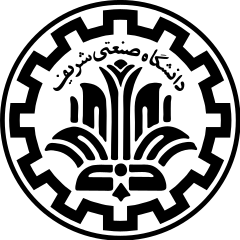
\includegraphics[scale=0.15]{Sharif}%\hfill \\[1em]  
	%\end{center}
	%\vspace{-3em}
\begin{center}

\bf
%\begin{outline} 
{
\LARGE
#1
}
%\end{outline} 
\\
تمرین #2
\end{center}
\vspace*{-1em}
\noindent
نام و نام‌خانوادگی: #3 \hfill شماره دانشجویی: #4
\vspace{-4mm}
\rule{\textwidth}{1pt}
%\ \\
}

% example environment
\newenvironment{example}
{\smallskip \noindent \emph{مثال:}}
{\hfill $\boxtimes$ \smallskip}

\def\Max{\text{بیشینه کن}}
\def\Min{\text{کمینه کن}}
\def\st{\text{\rl{که}}}

\newtheorem{theorem}{قضیه}
\newtheorem{proposition}{گزاره}
\newtheorem*{claim}{ادعا}
\newtheorem*{lemma}{لم}
\newtheorem{numlemma}{لم}
\newtheorem{corollary}{نتیجه}
\newtheorem*{definition}{تعریف} % Use this for non-trivial definitions.
 %%%%%%%%%%%%%%%%%%%%%%%%%%%%%%%%%%%%%%%%%%%%%%%%%%%%%%%%%%%%%%%%%%%%%%%%%%%%




\begin{document}

\exercise{5}{درخت فضایی}{آئیریا محمدی}
\section{}
\proof برهان خلف
فرض کنیم 
چنین آرایه‌ای را می‌توان در زمان خطی با الگوریتمی به اسم lin-sort مرتب کرد. 

الگوریتم زیر را 
تبدیل هر آرایه دلخواه به شکل مورد نظر ارائه می‌دهیم
\begin{latin}
\begin{codebox}
	\Procname{$f(B, n)$}
\li condition = true \Comment true for greater, false for smaller
\li	\For $i=1:n$ \Then
	\li \If condition and B[i] < B[i-1] \Then 
	\li	swap B[i], B[i-1]
	\End
	\li \If not condition and B[i] > B[i-1] \Then
	\li swap B[i], B[i-1]
	\End
	condition = not condition
	\End
\end{codebox}
\end{latin}

\paragraph{تحلیل زمانی الگوریتم}
 الگوریتم هر عضو از آرایه A را یک بار می‌بیند و در هر دور $O(1)$ عملیات انجام می‌دهد.
پس از 
$O(n)$ 
است.

\paragraph{درستی الگوریتم}
اثبات با استقرا.

برای $n=1$ درستی آن بدیهی است 
$(B = A = \{ x \})$
.

اگر برای آرایه‌های با اندازه کمتر از 
$n$
الگوریتم را درست فرض کنیم٫ برای آرایه به اندازه 
$n$
خواهیم داشت:
???

حال می‌توانیم هر آرایه دلخواه را با الگوریتم زیر مرتب کنیم:
\begin{latin}
\begin{codebox}
	\Procname{$sort(A, n)$}
	\li f(A, n)	\Comment O(n)
	\li lin-sort(A, n) \Comment O(n)
\end{codebox}
\end{latin}

\paragraph{تحلیل زمانی و درستی}
الگوریتم از مرتبه‌زمانی 
$O(n)$ 
است و درستی آن بنا بر درستی الگوریتم‌های استفاده شده و برقراری شرط مطرح شده درست است.

در حالی که می‌دانیم نمی‌توان چنین الگوریتمی با مرتبه زمانی کمتر از 
$O(n\cdot logn)$
داشت. 
پس فرض غلط است و الگوریتم 
lin-sort
نمی‌تواند وجود داشته باشد.

\newpage
\usetikzlibrary{positioning, decorations.text}
\section{}
دایره مورد نظر را به $n$ بخش با مساحت‌های مساوی تقسیم می‌کنیم.
مساحت هر بخش برابر با 
$ \pi (1^2)/n = \pi / n $
خواهد بود.
برای دایره مرکزی خواهیم داشت
\begin{equation}
	\pi r^2 = \pi / n \rightarrow r = \sqrt{1/n}
\end{equation}

و شعاع دایره ناحیه دوم برابر خواهد بود با
\begin{equation}
	\pi R^2 - \pi r^2 = \pi R^2 - \pi / n = \pi / n \rightarrow R = \sqrt{2/n}
\end{equation}

و برای هر ناحیه شماره $i$ داریم
$(r = r_{i-1}, R = r_i)$
\begin{equation}
	\pi R^2 - \pi r^2 = \pi / n \rightarrow R = \sqrt{\frac{1}{n} + r^2}
\end{equation}

تعریف:
$$r_i = \text{شعاع دایره i ام}$$

ادعا:
شعاع دایره محیطی ناحیه $i$ 
برابر است با 
$\sqrt{\frac{i}{n}}$

اثبات با استقرا:

برای پایه استقرا٫ صحت فرض را به ازای $i =2$ در بالا نشان دادیم٫
و فرض را برای 
$i-1$
دایره اول درست فرض می‌کنیم.

اثبات برای $i$
\begin{equation}
	R = \sqrt{\frac{1}{n} + r^2} = \sqrt{\frac{1}{n} + (\sqrt{\frac{i-1}{n}})^2}
	= \sqrt{\frac{1}{n}+\frac{i-1}{n}} = \sqrt{\frac{i}{n}}
\end{equation}

\begin{figure}
\centering
\begin{tikzpicture}[scale=1.0]
\draw [step=1.0,thin,gray!40] (-3,-6) grid (9,6);
\fill[blue] (3,0) circle (2pt) node [black,below left] {$C$};
\draw[thick] (3,0) circle(3);
\draw[thick] (3,0) circle(4);
\draw[thick] (3,0) circle(5);
\draw[thick] (3,0) circle(2);
\begin{scope}[>=latex]
\draw[->] (3,0) -- (5,0)  node [midway,fill=white] {$\sqrt{1/n}$};
\draw[->] (3,0) -- ++(45:3)  node [midway,sloped,fill=white] {$\sqrt{2/n}$};
\draw[->] (3,0) -- ++(-225:5)  node [midway,sloped,fill=white] {$\sqrt{n/n}$};
\end{scope}

\draw [decorate, decoration={text along path, text = second bucket, text align = center}] (0.5,0) arc (180:0:2.5 cm); 

\draw [decorate, decoration={text along path, text = n'th bucket, text align = center}] (-1,2.4) arc (150:60:4.5 cm); 

\draw [decorate, decoration={text along path, text = first bucket}] (2,-1) arc (-90:90:5); 
\end{tikzpicture}
\caption{دایره را به $n$ ناحیه با مساحت مساوی تقسیم کردیم}
\end{figure}

حال مسئله اصلی را حل می‌کنیم.

با توجه به فرض سوال٫ از آن‌جایی که متوسط تعداد نقاط در هر ناحیه متناسب با مساحت آن ناحیه است
اگر دایره را به ناحیه‌های هم مساحت تقسیم کنیم به طور میانگین در هر ناحیه یک نقطه خواهیم داشت.

اگر از الگوریتم
\lr{bucket sort}
استفاده کنیم:
\begin{equation}
	T(n) = \Theta(n) + \sum_{i=1}^n (n_i) ^ 2
\end{equation}

که 
$n_i$
تعداد نقاط در ناحیه 
$i$
است.

و اگر امید ریاضی مرتبه‌ زمانی را حساب کنیم
\begin{equation}
	E[T(n)] = E[\Theta(n) + \sum_{i=1}^n (n_i) ^ 2]
\end{equation}

بعد دو مرحله استفاده از خاصیت خطی‌بودن امیدریاضی
\begin{equation}
	E[T(n)] = E[\Theta(n)] + \sum_{i=1}^n E[n_i ^ 2]
\end{equation}

اگر تعریف کنیم
\begin{equation}
	X_{ij} = \begin{cases}
		1 & \mbox{
		point i being in area j
		} \\
		0 & \mbox{otherwise} 
	\end{cases}
\end{equation}

خواهیم داشت
\begin{equation}
	n_j = \sum_{i=0} ^n X_{ij} 
\end{equation}

پس
\begin{equation}
	E[n^2_i] = E[(\sum_{j=0} ^n X_{ji})^2] = E[\sum_{j=0} ^n X_{ji}^2] + E[\sum_{j=0} ^n \sum_{k=0} ^n 2 X_{ji} X_{ki}]
\end{equation}

برای بخش اول از آن‌جایی که احتمال وجود نقطه در هر ناحیط برابر و برابر با 
$\frac{1}{n}$
است داریم
\begin{equation}
	E[X^2_{ji}] = (1-\frac{1}{n}) * 0^2 + \frac{1}{n} * 1^2 = \frac{1}{n}
\end{equation}
\begin{equation}
	E[\sum_{j=0} ^n X_{ji}^2] = \sum_{j=0} ^n E[X_{ji}^2] = n \cdot \frac{1}{n} = 1
\end{equation}

و برای بخش دوم با توجه با استقلال
$X_{ji}$
و
$X_{ki}$
داریم
\begin{equation}
	E[\sum_{j=0} ^n \sum_{k=0} ^n 2 X_{ji} X_{ki}] = \sum_{j=0} ^n \sum_{k=0} ^n 2 E[X_{ji}] E[X_{ki}] = {n \choose 2} \cdot 2\cdot\frac{1}{n}\cdot \frac{1}{n} = \frac{n(n-1)}{n^2} = 1 - \frac{1}{n}
\end{equation}

و در نتیجه 
\begin{equation}
	E[n_i ^ 2] = 2 - \frac{1}{n}
\end{equation}

در نهایت خواهیم داشت
\begin{equation}
	E[T(n)] = E[\Theta(n)] + \sum_{i=1}^n 2 - \frac{1}{n} = 
	\Theta(n) + 2n - n(1/n) = \Theta(n) + O(n)
\end{equation}







%\exercise{6}{انتخاب سریع هرمی}{آئیریا محمدی}
%\proof
برهان خلف

فرض کنیم این‌گونه نباشد. یعنی بتوان نزدیک‌ترین عنصر آرایه 
$n$
عضوی 
$A$
به مقدار 
$x$
را در زمان 
$o(logn)$
٫ مثلا 
$O(1)$
پیدا کرد
.

آن‌گاه می‌توان الگوریتم زیر را برای مرتب کردن اعداد ارائه داد:
\lr{
\begin{codebox}
	\Procname{$\proc{sort}(A, n)$}
	\li list : LinkedList
	\li it = list.iterator : ListIterator
	\li list.add(A[0], it)  \Comment adds item to the list where iterator points, and iterator moves forward
	\li \For element 
\end{codebox}
}
%\exercise{7}{فقط چند تغییر}{آئیریا محمدی}
%%کپی شده و ادیت نشده%

%\begin{latin}
%\begin{codebox}
%	\Procname{$\proc{}$}
%	
%\end{codebox}	
%\end{latin}


یک درخت 
trie 
می‌سازیم با این تفاوت
که برای بچه‌های آن ترتیب 
قائل می‌شویم.
به عبارتی
اگر دو کلمه 
xb 
و 
xa 
را در آن اضافه کنیم درخت به یاد 
داشته باشد که بین بچه های 
x 
اول 
b 
بوده است و سپس 
a
.
حال تمام رشته ها را به این درخت اضافه می‌کنیم.
.

همچنین یک گراف جهت‌دار با H راس 
( هر راس نماینده یک حرف الفبا) 
می‌سازیم
.

حال بر روی این درخت ترای پیمایش می‌کنیم
(مثلا 
BFS
)
و برای هر گره‌که به آن می‌رویم این عملیات را انجام می‌دهیم
:

برای فرزندان گره مورد نظر:
نقاط متناظر حروف فرزاندان 
$i$ 
و
$i+1$
را در گراف ساخته شده پیدا می‌کنیم 
و
از فرزند چپی (کوچک‌تر) به راستی یک یال رسم می‌کنیم
.
این کار را برای هر دو جفت فرزند مجاور این گره انجام می‌دهیم.

مفهوم
 پشت کاری که انجام دادیم این است که اگر دو
 رشته تا تعدادی حرف مشابه باشند٫ 
 اولین حرفی که متفاوت هستند 
 به ما این آگاهی را می‌دهد 
 که آن حرف رشته کوچیک تر از حرف هم اندیسش در رشته بزرگ‌تر کوچک تر است
 و
  این روابط کوچک‌تری را در گراف می‌توان به راحتی نگهداری کرد.

همچنین نیازی نیست تمام رشته ها را دو به دو بررسی کرد چون کوچک‌تری خاصیت تعدی دارد و کافی است رشته های مجاور را مقایسه کرد.

  در نهایت بر روی گراف ساخته شده از ترتیب‌های جزئی در زمان 
O(?????????)
   توپولوژیکال سورت انجام می‌دهیم 
  و به یکی از جواب‌های درست مسئله دست میابیم
  .

  اگر در گراف ساخته شده دور وجود داشته باشد برای این مسئله جوابی وجود ندارد 
  و می‌توان در زمان ثابت 
  بر روی این گراف با راس‌های مشخص به دنبال دور گشت
  (با پیدا کردن یال های عقب گرد در 
  DFS
  ) .
  چرا که ارزش ترتیبی هیچ دو حرفی با هم مساوی نیست 
  و 
  از دور می‌توان نتیجه گرفت تمام حروف روی دور با هم مساوی و هم ارزش هستند
  .


  برای سورت توپولوژیک هم 
  به این شکل عمل می‌کنیم که الگوریتم 
  DFS 
  میزنیم اما با این فرق که 
  یک استک داریم و برای هر راسی 
  که به آن می‌رویم ابتدا 
  به طور بازگشتی برای تمام همسایه‌های آن 
  نیز  
  DFS
  را فراخوانی می‌کنیم 
  و
   سپس مقدار این گره را
   در استک وارد می‌کنیم.

   حال می‌توانیم اعضای استک را نوبتی بیرون بیاوریم
   که نشان دهنده ترتیب اعداد از کوچک به بزرگ می‌باشد
   .


   \paragraph{تحلیل زمانی}
   ساختن و پیمایش گراف در زمان ثابت انجام می‌شود.
    ساختن و پیمایش درخت ترای نیز در زمان
    تعداد کل حروف تمام کلمات
    که برابر با مجموع طول آن‌ها 
    (K) 
    انجام می‌شود.
    و برای هر گره ترای نیز باید 
    حداکثر
    ۲۶ 
    فرزند را 
    در ۲۷ 
    عملیات مقایسه کنیم 
    (یال متناظر در گراف اضافه کنیم)
    که این ضریبی برای هزینه پیمایش گره ترای می‌شود
    $(O(27K) = O(K))$

    در نتیجه مرتبه زمانی الگوریتم از 
    $O(K)$
    خواهد بود
    .


% گرافی جهت‌دار با ۲۶ راس (هر راس نماینده یک حرف) می‌سازیم.
% کلمات مجاور را دو به دو و به ترتیب مقایسه می‌کنیم و در هر جفت٫ اولین حرفی که از چپ یکسان ندارند نشان دهنده یک نامساوی هست که می‌توانیم در گرافمان به شکل یال از حرف کوچک‌تر به بزرگ‌تر نمایش می‌دهیم. 

% در نهایت توپولوژیکال سورت گراف را در می‌آوریم.
%\exercise{8}{مرتب‌سازی ادغامی چندتایی}{آئیریا محمدی}
%1-
بر روی عضو اول هر دو لیست یک اشاره‌گر در نظر بگیرید. در هر مرحله از اجرای الگوریتم مقادیری که این دو به آن‌‌ها اشاره می‌کنند را با هم مقایسه می‌کنیم و هر کدام که بزرگ تر بود اشاره‌گرش را به محل جدید می‌بریم (یک واحد به راست).
هرگاه یکی از اشاره‌گر ها به انتها رسید تمام اعضای باقی مانده لیست دیگر را پشت هم می‌نویسیم.

بدترین حالت وقتی رخ می‌دهد که هر دو اشاره‌گر در یک نوبت به انتها برسند.
یعنی 
$i = n-1$
و 
$j = n$
.

در هر دور از اجرای الگوریتم تا وقتی که هیچ کدام از اشاره‌گر ها به انتها نرسیده است باید برای تشخیص عضوی که باید در آرایه جدید بنویسیم یک مقایسه انجام بدهیم. این کار تا وقتی انجام می‌شود که بالاخره یکی از اشاره‌گر ها به انتها برسد. سپس هرچه باقی مانده چیده می‌شود.
در بدترین حالت تنها یک عضو (عضو اخر آرایه دیگر) است که بدون نیاز به مقایسه گذاشته می‌شود. به عبارتی
$2n-1$
مقایسه انجام شده است.

سودوکد الگوریتم مطرح شده در زیر آمده است.

\begin{latin}
\begin{codebox}
	\Procname{$\proc{merge}(A, B, n)$}
	\li $i,j,x$ : int = 0
	\li B : List[int] of size $2n$
	
	\li \While $i<n$ or $j<n$ \Then
	\li \If $i = n$ \Then
		\li B[x] = A[j]
		\li j = j+1
	\li \Else \If $j = n$
		\li B[x] = A[i]
		\li i = i+1
	\li \Else \If A[i] < A[j]
		\li B[x] = A[i]
		\li i = i + 1
	\li \Else
		\li B[x] = A[j]
		\li j = j+1
	\End
	\li x = x+1
	\End
	
\end{codebox}
\end{latin}
\newpage
2-
برای ادغام کردن $k$ لیست کافی است آن‌ها را دو به دو با هم ادغام کنیم. سپس لیست‌های جدید را دوباره با هم دو به دو ادغام کنیم تا وقتی که تنها یک لیست داشته باشیم. 
%(اگر k فرد باشد با ایجاد اندکی تغییر در الگوریتم می‌توان دو لیست با اندازه های غیر همسان هم ادغام کرد)

اگر k زوج باشد مرتبه زمانی الگوریتم مطرح شده به شکل زیر خواهد بود:
\begin{equation*}
	T(nk) = T(nk/2) + O(2 \frac{nk}{2}-1)
\end{equation*}

%اگر k فرد باشد برای راحتی کار تعداد لیست ها را k+1 
%در نظر می‌گیریم

رابطه بالا از آن‌جا ناشی می‌شود که الگوریتم ما در عمل مانند این است که خود k دسته را ابتدا دو گروه کنیم و این الگوریتم را بر روی هر گروه اعمال کنیم و سپس دو ابرلیستی که تشکیل می‌شود را ادغام کنیم.

بدون ایجاد اشکال در جواب می‌توانیم فرض کنیم که k به شکل $2^m$
است. اگر این چنین نباشد 
$(2^{m-1} < k < 2^m)$
کافی است که 
$2^m - k$
لیست با تعداد $n$ 
عضو با مقدار مثلا منفی بی‌نهایت اضافه کنیم و در نهایت که به پاسخ رسیدیم تمام این عضوهای زائد را از چپ حذف کنیم (در $O(nk)$) 

و محاسبه می‌شود:
\begin{equation*}
	T(nk) = O(nk\cdot log(nk))
\end{equation*}

3-
فرض کنیم زمان آن قابل کاهش باشد.
به عبارتی 
$T(nk) = o(nk\cdot log(nk))$
.

کافی است قرار دهیم
$n= 1$
.
خواهیم داشت:
\begin{equation*}
	T(k) = o(k \cdot log k)
\end{equation*}

این به این معنا است ما می‌توانیم برای مرتب کردن 
$n$ 
عدد به این شکل عمل کنیم که در 
$O(n)$
هر عدد را در یک لیست خالی قرار دهیم و سپس این $n$ لیست بدیهتا مرتب را با هم در 
$ o(nlogn)$
ادغام کنیم.
در حالی که می‌دانیم همچین چیزی نمی‌تواند ممکن باشد که الگوریتم سورت با زمان قطعی کمتر از $O(n log n)$ 
داشت 	پس فرض غلط است.

%
\newpage
\section{عنوان بخش}
شروع بحث جلسه فعلی. 

پاراگراف‌ها با یک خط خالی از هم جدا می‌شوند. لازم نیست بین هر دو پاراگراف از \verb|\par|  استفاده کنیم.

می‌توانید برای نوشتن فرمول چندخطی می‌توانید از محیط \verb|align| استفاده کنید:
\begin{align*} 
\min \quad \| f \|_{\infty}\\ 
f \in F_{s,t} 
\end{align*}

سعی کنید قواعد نگارش فارسی را رعایت کنید. از نیم‌فاصله
به درستی استفاده کنید. علامت نقل قول در فارسی بدین صورت است «». پس از نقطه و ویرگول و دونقطه و پرانتزبسته‌ای که قبل از نقطه نیست و این‌گونه علامت‌ها، یک فاصله بگذارید.

خوب است معادل انگلیسی اصطلاحات را در پاورقی%
\LTRfootnote{footnote}
بیاورید.

برای نوشتن انگلیسی در میان متن فارسی، از دستور \verb+\lr{}+ استفاده کنید. 
مثلا:
\lr{Some English text here} 
در میان متن درست می‌آید.

استفاده از تاکید به صورت 
\textbf{پررنگ}
کردن یا 
\textit{ایتالیک}
کردن مفید است. 

برای شبه کدها از پکیج
\lr{clrscode3e}
استفاده کنید. برای آشنایی با این پکیج
\lr{clrscode.pdf}
را مطالعه کنید.


\section{محیط‌های مختلف}
\begin{lemma}
	یک لم.
\end{lemma}
\begin{theorem}
	\label{thm:sample}
	یک قضیه. 
\end{theorem}
\begin{proof}
	بدیهی.
\end{proof}

\begin{example}
	یک مثال. 
\end{example}

ارجاع به قضیه 
\ref{thm:sample}.

ارجاع به مراجع
\cite{lecture1}
و
\cite{CLRS}.

%برای قاطی نشدن متن فارسی و انگلیسی از
% Enter
%  زیاد استفاده کنید!

\bibliographystyle{alpha}

\begin{thebibliography}{99}
	\bibitem{lecture1}
	جزوه جلسه اوّل
	\bibitem{dr. ghodsi}
	قدسی، محمّد. \textit{داده ساختارها و مبانی الگوریتم‌ها}. تهران: فاطمی، ۱۳۹۵
	
	\begin{latin}	%english reference
		
		%book in MLA style: https://owl.purdue.edu/owl/research_and_citation/mla_style/mla_formatting_and_style_guide/mla_works_cited_page_books.html
		\bibitem{CLRS}
		Cormen, Thomas H., et al.
		\textit{Introduction to Algorithms}. 
		3rd ed., MIT Press, 2009, pp. 18-22. %page numbers
	\end{latin}	
\end{thebibliography}


\end{document}
